
\documentclass{article}
\usepackage{graphicx}
\usepackage{verbatim}
\usepackage[utf8]{inputenc}
\usepackage{ifthen}
\title{Fraud Detection Project: 10 Academy KAIM Week 8 \& 9}
\author{Bereket Feleke}
\date{August 2025}
\begin{document}
\maketitle

\section{Introduction}
This report presents the results of the fraud detection project for the 10 Academy KAIM Week 8 \& 9 Challenge, focusing on e-commerce and bank transaction fraud detection.

\section{Exploratory Data Analysis}
EDA was performed on the Creditcard and Fraud datasets. Key visualizations include:

\begin{figure}[h]
\centering
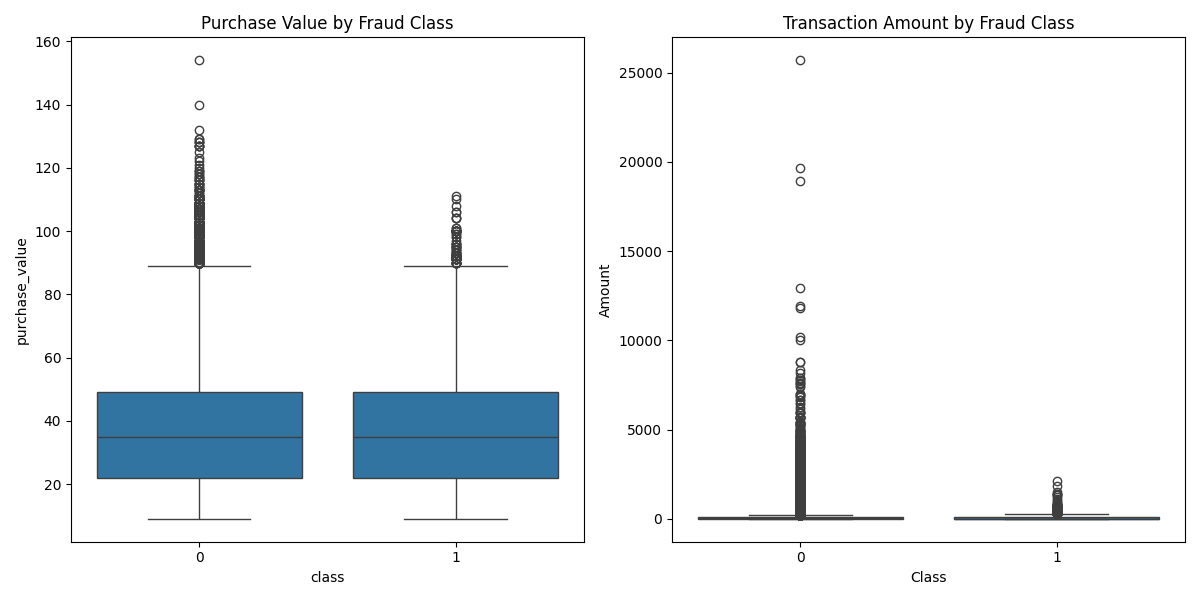
\includegraphics[width=0.5\textwidth]{/content/drive/MyDrive/reports/eda/bivariate_boxplots.png}
\caption{Bivariate boxplots showing feature relationships.}
\end{figure}

\begin{figure}[h]
\centering
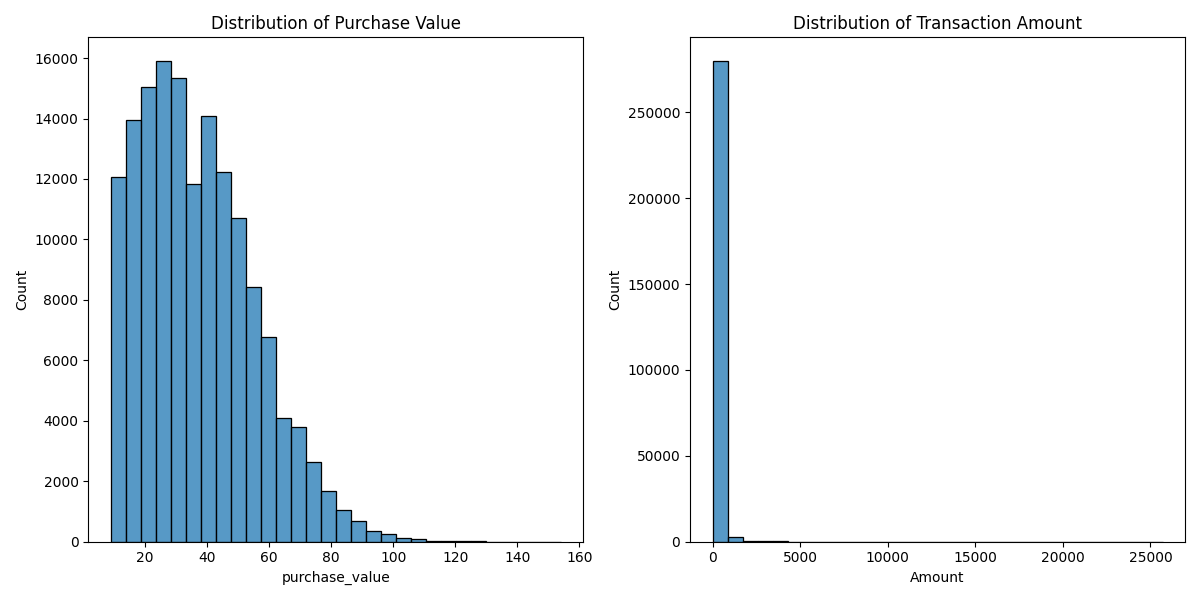
\includegraphics[width=0.5\textwidth]{/content/drive/MyDrive/reports/eda/univariate_distributions.png}
\caption{Univariate distributions of key features.}
\end{figure}

\section{Model Performance}
\footnotesize
\verbatiminput{/content/drive/MyDrive/reports/model_results.txt}

\begin{figure}[h]
\centering
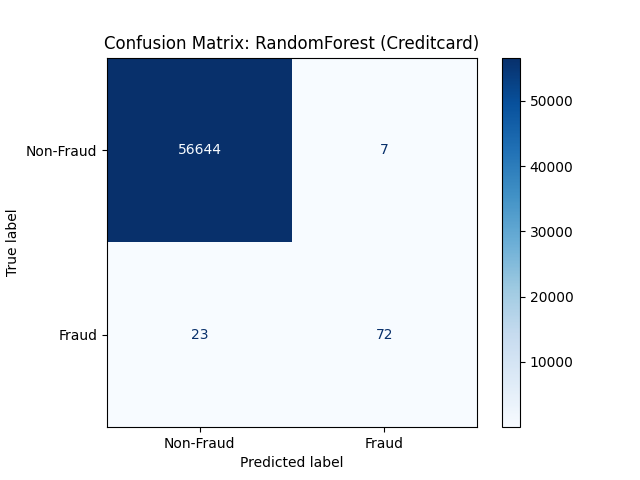
\includegraphics[width=0.3\textwidth]{/content/drive/MyDrive/reports/confusion_matrices/RandomForest_Creditcard_cm.png}
\caption{Random Forest confusion matrix for Creditcard dataset.}
\end{figure}

\begin{figure}[h]
\centering
\includegraphics[width=0.3\textwidth]{/content/drive/MyDrive/reports/confusion_matrices/LogisticRegression_Creditcard_cm.png}
\caption{Logistic Regression confusion matrix for Creditcard dataset.}
\end{figure}

\section{SHAP Analysis}
SHAP analysis was performed on the Random Forest model for the Creditcard dataset.

\begin{figure}[h]
\centering
\includegraphics[width=0.5\textwidth]{/content/drive/MyDrive/reports/shap/summary_plot_Creditcard.png}
\caption{SHAP summary plot for Creditcard dataset.}
\end{figure}

\IfFileExists{/content/drive/MyDrive/reports/shap/force_plot_Creditcard_instance_0.png}{%
\begin{figure}[h]
\centering
\includegraphics[width=0.5\textwidth]{/content/drive/MyDrive/reports/shap/force_plot_Creditcard_instance_0.png}
\caption{SHAP force plot for a sample instance in Creditcard dataset.}
\end{figure}
}{\textbf{Note}: SHAP force plot is provided as an HTML file (force_plot_Creditcard_instance_0.html) due to rendering limitations.}

\IfFileExists{/content/drive/MyDrive/reports/shap/shap_insights.txt}{%
\section{SHAP Insights}
\footnotesize
\verbatiminput{/content/drive/MyDrive/reports/shap/shap_insights.txt}
}{}

\section{Conclusion}
The Random Forest model was selected for its superior performance. SHAP analysis highlighted key features (e.g., V4, V14, V10) driving fraud predictions.

\end{document}
